\pagebreak
\chapter{CPU Scheduling} \label{CPU scheduling}
In questa sezione ci occupiamo di tutti gli aspetti che concernono lo scheduling del processore, ovvero la pratica secondo la quale, attraverso dei precisi criteri, si sceglie quale processo all'interno della \textit{ready queue} verrà eseguito.

\section{Nozioni fondamentali}
Prima di iniziare a discutere di scheduling vero e proprio è necessario avere chiari alcuni concetti importanti.

\paragraph{Burst.}
La prima è la nozione di burst. Chiamiamo \textbf{CPU burst} il periodo di tempo nel quale un processo esegue operazioni all'interno della CPU; diversamente, l'\textbf{I/O burst} è il tempo che il processo spende interfacciandosi con le periferiche di input e output. In particolare, un processo che occupa per molto tempo la CPU si dice \textit{CPU bounded}, mentre nel caso di I/O si parla di un processo \textit{I/O bounded}. In questo capito ci occupiamo solo di CPU burst.
% 
\paragraph{CPU scheduler.}
Il CPU scheduler è il responsabile dell'organizzazione e dell'ordinamento della \textbf{coda dei processi} (figura \ref{fig:process'life}). Le decisioni su quale processo deve essere eseguito prima stanno a lui. Questo tipo di decisioni avvengono generalmente quando un processo:
\vspace{-5px}
\begin{enumerate}
\setlength{\itemsep}{-.15 em}
    \item Passa dallo stato \textit{running} a \textit{waiting};
    \item Passa da \textit{running} allo stato \textit{ready};
    \item Passa dallo stato \textit{waiting} allo stato \textit{ready};
    \item Termina.
\vspace{-5px}
\end{enumerate}
Osserviamo che per i punti 1 e 4 non è presente una vera e propria decisione: un nuovo processo deve essere messo in esecuzione. Questo non vale per i punti 2 e 3 dove si fa una decisione.
\begin{figure}[h]
    \centering
    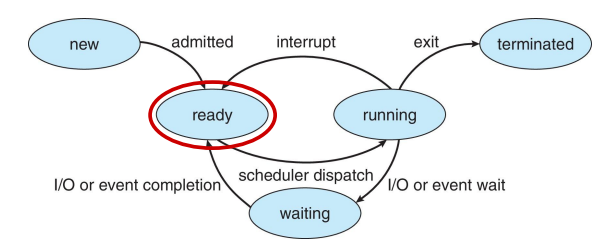
\includegraphics[width = .65\textwidth]{../res/imgs/CPU scheduling/dispatcher.png}
    \caption{Lo scheduler entra in gioco nel passaggio da ready a running.}
    \label{fig:process'life}
\end{figure}
% 
\paragraph{Preemption.}
Ci sono due macro gruppi di scheduling: preemptive e non. Uno scheduling è detto \textbf{non preemptive} nel momento in cui un processo non può essere fermato. In altre parole, quando la CPU è assegnata ad un processo, questo la utilizza fino a che non è terminato. Differentemente, uno scheduling è detto \textbf{preemptive} quando un processo può essere fermato per dare precedenza ad un altro per poi essere fatto ripartire: questo tipo di scheduling è sicuramente più performante e moderno; è infatti utilizzato nei sistemi operativi più diffusi come Windows, MacOS, Linux e altri. Ciò porta comunque a delle situazioni indesiderate come le \textbf{race conditions}: poniamo il caso di avere due processi che condividono dei dati; immaginiamo che il primo processo stia aggiornando questi dati ma allo stesso tempo il secondo processo li stia utilizzando. Questo è un problema dato che il processo due sta utilizzando dei dati che non sono consistenti dato che sono in fase di aggiornamento dal processo uno. Come vedremo nel capitolo \ref{sincronizzazione}, questo è un problema di sincronizzazione che va risolto.
% 
\paragraph{Dispatcher.}
Nel momento in cui lo scheduler ha scelto quale processo verrà eseguito, il dispatcher si occupa di cambiare il processo nella CPU. In particolare viene effettuato il \textit{context switch} (\ref{context_switch}), passa in \textit{user mode} e va alla giusta locazione del programma per iniziare la sua esecuzione. Durante tutto ciò la CPU però non lavora: è importante quindi minimizzare questa latenza e fare in modo che non se ne effettuino un numero troppo elevato al fine di mantenere un alta percentuale di utilizzo della CPU.
% 
\section{Algoritmi non preemptive}
In questo paragrafo ci occupiamo dei primi algoritmi non preemptive, ovvero gli algoritmi che non fermano i processi che sono in esecuzione. 

\subsection{First-Come First-Served (FCFS)}
Questo è l'algoritmo più banale da implementare: il primo processo che entra nella coda sarà anche il primo ad essere eseguito. Questo algoritmo ha un approccio praticamente identico al \textbf{FIFO} (\textit{First In First Out}). Attraverso un semplice esempio, possiamo osservare che questo algoritmo non è efficiente. Poniamo che entrino nella coda 3 processi: $P_1$, di durata 24 unità di tempo (in genere millisecondi) e $P_2$ e $P_3$ con durata di esecuzione 3.  
\begin{figure}[h]
    \centering
    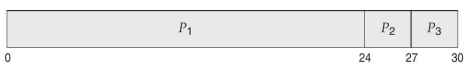
\includegraphics[width = .7\textwidth]{../res/imgs/CPU scheduling/FCFS.png}
    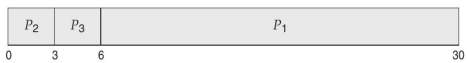
\includegraphics[width = .7\textwidth]{../res/imgs/CPU scheduling/FCFS2.png}
    \caption{Diagramma di \textit{Gantt} dell'algoritmo FCFS.}
    \label{fig:FCFS}
\end{figure}
Osservando la figura \ref{fig:FCFS} è banale notare che se $P_1$ fosse arrivato in coda per ultimo, i processi $P_2$ e $P_3$ avrebbero aspettato meno.
Possiamo dimostrarlo anche in maniera più matematica, attraverso dei brevi calcoli. Nel primo caso $P_1$ ha aspettato 0 prima di essere eseguito, $P_2$ ha aspettato l'esecuzione di $P_1 = 24$ mentre $P_3$ ha aspettato l'esecuzione di $P_1 + P_2 = 24 + 3 = 27$. Se provassimo a fare una media del tempo di attesa otteniamo:
\begin{gather*}
    \langle T\rangle = \frac{0 + 24 + 27}{3} = 17
\end{gather*}
Nel secondo caso invece la situazione migliora notevolmente in quanto $P_2$ aspetta 0, $P_3$ aspetta solamente l'esecuzione di $P_2 = 3$ e infine $P_1$ attende l'esecuzione di $P_2 + P_3 = 3 + 3 = 6$. Attraverso la stessa espressione matematica otteniamo che l'attesa media in questo caso diventa:
\begin{gather*}
    \langle T \rangle = \frac{6 + 0 + 3}{3} = 3
\end{gather*}

Diversi sono i problemi di questo algoritmo. Prima di tutto può generare il \textbf{convoy effect} (effetto convoglio): se viene eseguito un processo \textit{I/O bounded}, tutti gli altri processi in coda devono aspettare che questo si "sblocchi" generando quindi un rallentamento generale. In secondo luogo, questo algoritmo di scheduling dipende dall'ordine di entrata dei processi e di conseguenza \textbf{non} è nemmeno possibili analizzare in modo \textbf{deterministico} le prestazioni dell'algoritmo.
% 
\subsection{Shortest-Job-First (SJF)}\label{SJF}
Come abbiamo notato dalla figura \ref{fig:FCFS}, se i processi più bervi sono eseguiti prima, il tempo medio di attesa $\langle T \rangle$ si abbassa. Implementiamo quindi un algoritmo che dia la precedenza ai processi con il tempo di esecuzione più breve tra quelli che sono presenti in coda. In questo algoritmo stiamo assumendo che siamo a conoscenza del CPU burst time di ciascun processo: si osserva che stiamo facendo un'ipotesi, spesso questo dato non è a disposizione. Se tutti i CPU burst sono conosciuti, l'algoritmo fornisce il minor tempo medio di attesa di un insieme finito di processi.

Il funzionamento di questo algoritmo è molto semplice: in base ai processi arrivati in coda, questi, prima di essere eseguiti, vengono riordinati in base al loro tempo di burst. Per esempio, poniamo di avere in coda un processo $P_1$ con un burst time di 6, $P_2$ da 8, $P_3$ da 7 e $P_4$ da 3.
\begin{figure}[h]
    \centering
    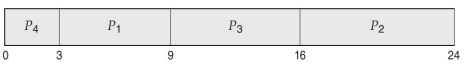
\includegraphics[width = .7\textwidth]{../res/imgs/CPU scheduling/SJF.png}
    \caption{Diagramma di \textit{Gantt} dell'algoritmo SJF.}
    \label{fig:SJF}
\end{figure}
Osservando la figura \ref{fig:SJF} notiamo che i processi sono stati riordinati in modo tale da minimizzare il tempo medio d'attesa. In questo esempio il processo $P_4$ attende 0, il processo $P_1$ attende l'esecuzione di $P_4 = 3$, il processo $P_3$ aspetta la conclusione di $P_4 + P_1 = 3 + 6 = 9$ e infine il processo $P_2$ aspetta $P_4 + P_1 + P_3 = 3 + 6 + 7 = 16$. Ecco che il tempo di attesa medio diventa:
\begin{gather*}
    \langle T \rangle = \frac{3 + 16 + 9 + 0}{4} = 7
\end{gather*}

Anche in questo caso però se durante l'esecuzione è in coda un processo con un burst molto alto e entrano solo processi con un burst basso, è probabile che si verifichi una situazione di attesa perenne (chiamata \textbf{starvation}); vedremo, nel corso di questo capitolo, come ciò può essere evitato (\ref{priority scheduling}).
% 
\subsection{Stima del \textit{CPU burst time}}
Come abbiamo affermato poco fa, quasi mai il burst time è a disposizione. Si è quindi trovato un modo per stimare al meglio il burst time di un processo, in base ai processi che sono stati eseguiti in precedenza. Il metodo utilizzato è chiamato \textbf{exponential averaging} il quale, in essenza, dà peso maggiore ai processi eseguiti da poco tempo e, pian piano, più i processi sono remoti, meno influenza hanno sulla stima. Le variabili in gioco nella formula sono:
\vspace{-5px}
\begin{itemize}
\setlength{\itemsep}{-.15 em}
    \item $t_i$ indica la durata del CPU burst del processo \textit{i}-esimo, dove $i\in[0,n]$, dove $n$ indica il numero di processi;
    \item $\tau_{n+1}$ rappresenta la stima, la predizione (\textit{guess}), che si calcola sul processo che si sta per eseguire;
    \item $\alpha$ che è un coefficiente che indica quanto pesa la storia dei processi. Quando questo coefficiente è basso, la storia recente non conta, mentre quando è alto, la storia recente ha più peso (con $\alpha = 1$ si ha che solo l'ultimo processo influisce sulla stima). Generalmente si utilizza il valore $\alpha = \frac{1}{2}$.
\end{itemize}
Nel caso generale, con $n$ processi si ha che per stimare il burts dell' $n+1$-esimo:
\begin{gather*}
    \tau_{n + 1} = \alpha t_n + (1 - \alpha)\alpha t_{n - 1} + ... \\
                    + (1 - \alpha)^i\alpha t_{n - i} + ...\\
                    + (1 - \alpha)^{n + 1}\tau_0
\end{gather*}

Osserviamo ora la figura \ref{fig:CPU burst estimation} che rappresenta come viene effettuata la \textit{guess} in base alla storia dei processi ($\alpha = .5$).
\begin{figure}[h]
    \centering
    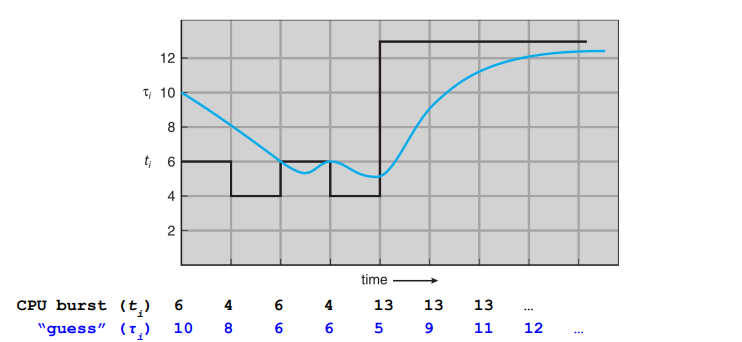
\includegraphics[width = .75\textwidth]{../res/imgs/CPU scheduling/CPU_burst_estimation.png}
    \caption{Grafico che indica come viene stimato il burst di un processo.}
    \label{fig:CPU burst estimation}
\end{figure}
La prima colonna composta dalla coppia $\binom{6}{10}$ è la colonna "base", la partenza del nostro grafico. Con questi due dati, si calcola la seconda colonna $\binom{4}{8}$, dove $ 8 = \frac{10 + 6}{2}$; a questo punto si può calcolare la terza colonna $\binom{6}{6}$, dove il secondo $6 = \frac{4 + 8}{2}$. Così facendo si è in grado di calcolare una buona stima per il CPU burst time del processo corrente.

% 
\section{Algoritmi preemptive}
In questo secondo paragrafo discutiamo invece di due algoritmi preemptive, ovvero algoritmi che possono fermare l'esecuzione di un processo per favorirne un altro.

% 
\subsection{Shortest-Remaining-Time-First (SRTF)}
Il primo algoritmo che andremo a discutere è la versione preemptive del SJF: in questo caso viene servito per primo il processo al quale manca minor tempo per essere completato. Quindi se si sta eseguendo un processo $P$ e arriva un processo $Q$ il quale burst time è minore rispetto al burst time che manca a $P$ per terminare, quest'ultimo viene fermato per dare la precedenza a $Q$. Una volta terminata l'esecuzione di $Q$, il processo $P$ riprede da dove era stato fermato in precedenza. Prendiamo in considerazione i seguenti 4 processi:
\begin{table}[h]
    \centering
    \begin{tabular}{c c c}
        \textbf{Processo} & \textbf{Tempo di arrivo} & \textbf{Stima burst time} \\\hline
        $P_1$ & 0 & 8 \\
        $P_2$ & 1 & 4 \\
        $P_3$ & 2 & 9 \\
        $P_4$ & 3 & 5 \\\hline
    \end{tabular}
\end{table}

Osservando la figura \ref{fig:SRTF}, cerchiamo di capire come si comporta questo algoritmo nel momento in cui i 4 processi sono inseriti all'interno della coda.
\begin{figure}[h]
    \centering
    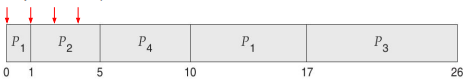
\includegraphics[width = .75\textwidth]{../res/imgs/CPU scheduling/SRTF.png}
    \caption{Diagramma di \textit{Gantt} dell'algoritmo SRTF.}
    \label{fig:SRTF}
\end{figure}
Al tempo zero arriva in coda il processo $P_1$, di durata 8. Al tempo 1 arriva in coda il processo $P_2$ che ha una durata di 4. A $P_1$ rimangono ancora $8 - 1 = 7$ unità di tempo prima di terminare, mentre a $P_2$ ne servono solo 4. $P_1$ viene quindi fermato e $P_2$ inizia la sua esecuzione (si effettua un \textit{depatching}). Al tempo 2 e al tempo 3 sono aggiunti alla coda $P_3$ e $P_4$ i quali però hanno un burst time maggiore rispetto a $P_2$ che quindi termina l'esecuzione al tempo $1 + 4 = 5$. A questo punto rimangono $P_1$, $P_3$ e $P_4$. Viene eseguito $P_4$ in quanto il suo burst (5) è minore rispetto a quello di $P_1$ (7) e $P_3$ (9). Terminata l'esecuzione di $P_4$ inizia quella di $P_1$ e poi quella di $P_3$.

Osserviamo che con questo algoritmo può capitare che sia in esecuzione un processo con un tempo di burst molto elevato e che poi continuino ad arrivare dei processi con un tempo di burst ridotto. In questo caso, il processo con il tempo maggiore verrebbe sempre interrotto dagli altri processi e non riuscirebbe mai a terminare andando quindi in una situazione di \textbf{starvation}. Come vedremo, una soluzione è questo problema è fornita dallo scheduling con priorità (\ref{priority scheduling}).

% 
\subsection{Round Robin (RR)}\label{RR}
Passiamo ora ad un algoritmo un po' più sofisticato ed elegante: stiamo parlando del Round Robin. Alla base di questo algoritmo c'è il \textbf{quanto} di tempo (generalmente tra i 10 e i 100 millisecondi): ogni processo all'interno della coda, ha diritto ad essere eseguito per 1 quanto di tempo alla volta. Di conseguenza, ogni quanto di tempo viene effettuato un \textit{context switch} e si prosegue ad un altro processo nella coda: si continua così in maniera ciclica finché ciascun processo viene eseguito completamente lasciando spazio ai nuovi.

Osserviamo che se $q \to\infty$ si ha un comportamento FIFO, molto simile all'algoritmo First-Come First-Served. Allo stesso tempo però $q$ deve comunque essere maggiore del tempo che ci si impiega per effettuare un context switch (ordine dei $\mu s$), altrimenti la CPU viene sprecata solo per fare i context switch al posto di effettivamente eseguire i processi. 

Consideriamo il caso in cui $q = 4$ e in coda sono presenti i tre processi utilizzati nell'algoritmo FCFS:
\begin{table}[h]
    \centering
    \begin{tabular}{c c}
        \textbf{Processo} & \textbf{Stima burst time} \\\hline
        $P_1$ & 24 \\
        $P_2$ & 3 \\
        $P_3$ & 3 \\\hline
    \end{tabular}
\end{table}

\noindent Il comportamento del Round Robin, in questo caso, è illustrato nella figura \ref{fig:RR}.
\begin{figure}[h]
    \centering
    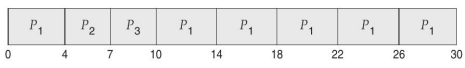
\includegraphics[width = .75\textwidth]{../res/imgs/CPU scheduling/RR.png}
    \caption{Diagramma di \textit{Gantt} dell'algoritmo RR.}
    \label{fig:RR}
\end{figure}
Osserviamo che il RR, per il processo $P_1$, ogni $q = 4$, si ferma per fare spazio agli altri processi mentre, per i processi $P_2$ e $P_3$, che durano meno di un quanto, quando terminano il Round Robin, non aspetta la scadenza del quanto per eseguire un altro processo ma comincia subito, che è un comportamento ragionevolmente ovvio. 
% 
\subsection{Reattività}
Cerchiamo ora di capire il vantaggio che forniscono gli algoritmi di scheduling preempitive (in particolare il RR) rispetto agli algoritmi non preemptive. Prendiamo come esempio i seguenti processi:
\begin{table}[h]
    \centering
    \begin{tabular}{c c}
        \textbf{Processo} & \textbf{Burst time} \\\hline
        $P_1$ & 6 \\
        $P_2$ & 3 \\
        $P_3$ & 1 \\\
        $P_4$ & 7 \\\hline
    \end{tabular}
\end{table}

\noindent Poniamo ora che il quanto di tempo \textit{q} sia 4. Calcoliamo ora il tournaround time medio tra questi processi: $P_1$ viene eseguti per 4 unità, dopo di chè viene fermato (gliene rimangono 2) e viene eseguito $P_2$ che terima ($T_{P_2}$ = 4 + 3 = 7); viene quindi eseguito $P_3$ che termina anche lui ($T_{P_3}$ = 7 + 1 = 8). A questo punto inizia l'esecuzione di $P_4$ che viene fermato dopo 4 unità (ne rimangono ancora 3) e viene fatto ripartire $P_1$ che termina ($T_{P_1}$ = 8 + 4 + 2 = 14) e infine viene fatto terminare anche $P_4$ ($T_{P_4}$ = 14 + 3 = 17). Per trovare il turnaround time medio si effettua la media dei 4 tournaround trovati.
\begin{gather*}
    \langle T \rangle = \frac{ T_{P_1} + T_{P_2} + T_{P_3} + T_{P_4}}{4} = \frac{14 + 7 + 8 + 17}{4} = \frac{46}{4} = 11.5
\end{gather*}

Osserviamo però che se avessimo utilizzato l'algoritmo SJF (vedi \ref{SJF}) il tournaround time medio è 8 che è minore rispetto a quello fornito da RR. Ciò significa che utilzzare un algoritmo pre-emptive, in termini di tempistiche, non è necessariamente la scelta migliore, è semplicemente un altro modo per schedulare l'esecuzione dei processi, ma non ne garantisce il miglioramento della prestazione. Allora perchè utilizzare questi algoritmo? Perchè migliora la reattività (\textbf{responsiveness}) del sistema. Ipotizziamo di avere un coda moltissimi processi che stanno in esecuzione. Un algoritmo non preempitve li esegue uno ad uno (secondo determinati criteri, più o meno efficienti) ma tutti i processi devono sempre stare in attesa che uno termini. Il RR invece garantisce che tutti i processi vengano eseguiti per almeno un certo quanto \textit{q} di tempo: è quindi un algoritmo più \textbf{equo} rispetto agli algoritmi non preemptive.

% 
\section{Scheduling con priorità} \label{priority scheduling}
Fino ad ora abbiamo trattato i processi in modo equo se non per la stima del \textit{burst time}. Introduciamo ora una seconda informazione, la \textbf{priorità} che non è altro che un numero che indica quanto sia importante (urgente) l'esecuzione di un determinato algoritmo. La priorità può essere sia legata al CPU burst time ma può anche essere legata ad altri aspetti. 

Arriva però un problema: la \textbf{starvation}. Anche in questo caso, come nel SRTF, può capitare che i processi che hanno una priorità di grado molto basso non vengano mai eseguiti in quanto sono sempre presenti processi con una priorità più alta. Con l'introduzione della priorità però, se un processo è da troppo tempo in coda, si aumenta di un grado la priorità al fine da mandarlo in esecuzione. Questa tecnica rappresenta allegoricamente l'invecchiamento (\textbf{aging}) del processo nella coda di attesa. 

Vediamo ora un primo esempio di scheduling con priorità puro. Abbiamo a che fare con i 5 processi seguenti:
\begin{table}[h]
    \centering
    \begin{tabular}{c c c}
        \textbf{Processo} & \textbf{Stima burst time} & \textbf{Priorità} \\\hline
        $P_1$ & 10 & 3 \\
        $P_2$ & 1 & 1 \\
        $P_3$ & 2 & 4 \\
        $P_4$ & 1 & 5 \\
        $P_5$ & 5 & 2 \\\hline
    \end{tabular}
\end{table}

\noindent Osserviamo che noi consideriamo come numero più basso la priorità più alta (di conseguenza $P_2$ è il processo con priorità più alta e $P_4$ quello con priorità più bassa). Detto ciò procediamo con il diagramma di Gantt (figura \ref{fig:priority_scheduling}).
\begin{figure}[h]
    \centering
    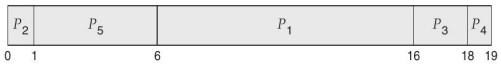
\includegraphics[width = .75\textwidth]{../res/imgs/CPU scheduling/priority_scheduling.png}
    \caption{Diagramma di \textit{Gantt} dell'algoritmo basato puramente sulla priorità.}
    \label{fig:priority_scheduling}
\end{figure}
Notiamo infatti che i processi sono eseguiti in ordine in base alla loro priorità: $P_2, P_5, P_1, P_3$ e $P_4$. Ovviamente, se durante l'esecuzione di $P_1$ (che ha priorità 3) fosse arrivato in coda un algoritmo con priorità 2, $P_1$ sarebbe stato interrotto per favorire l'esecuzione del nuovo processo. Inoltre, nel caso in cui due processi abbiano la stessa priorità si segue la dinamica FIFO, ovvero il primo processo che entra nella coda viene eseguito per primo rispetto ai processi con medesima priorità

% 
\subsection{Scheduling con prirità e RR}
Cerchiamo ora di raffinare un po' di più l'algoritmo fondendo la priorità con l'algoritmo di Round Robin. In particolare, nel momento in cui si hanno più processi che hanno lo stesso livello di priorità, al posto di seguire un approccio FIFO, si utilizza il Round Robin, garantendo quindi una maggiore reattività ai processi. Partiamo dal seguente set di processi:
\begin{table}[h]
    \centering
    \begin{tabular}{c c c}
        \textbf{Processo} & \textbf{Stima burst time} & \textbf{Priorità} \\\hline
        $P_1$ & 4 & 3 \\
        $P_2$ & 5 & 2 \\
        $P_3$ & 8 & 2 \\
        $P_4$ & 7 & 1 \\
        $P_5$ & 3 & 3 \\\hline
    \end{tabular}
\end{table}

\noindent Come è possibile osservare dalla figura \ref{fig:priority_RR}, notiamo che il processo 4, essendo che è l'unico processo con priorità 1, viene eseguito per primo e non viene interrotto da nessun'altro processo.
\begin{figure}[h]
    \centering
    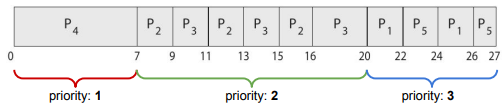
\includegraphics[width = .75\textwidth]{../res/imgs/CPU scheduling/priority_RR.png}
    \caption{Diagramma di \textit{Gantt} dello scheduling con priorità unito all'algoritmo RR per i processi con lo stesso grado di urgenza.}
    \label{fig:priority_RR}
\end{figure}
Dopo di che si effettua l'algoritmo RR con \textit{q} = 2 sui processi 2 e 3 in quanto hanno la stessa priorità. Infine, si fa lo stesso procedimento che con i processi 1 e 5 che hanno priortà 3. 

% 
\subsection{Coda multilivello}
\begin{wrapfigure}{o}{.25\textwidth}
  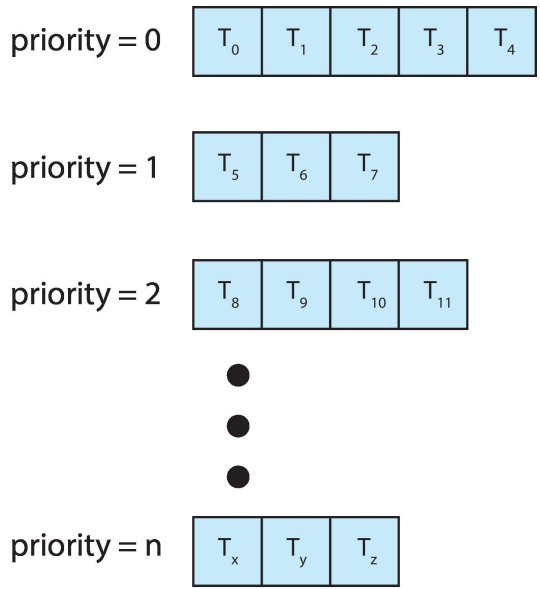
\includegraphics[width = \linewidth]{../res/imgs/CPU scheduling/multilevel_scheduling.png}
  \label{fig:multilevel_scheduling}
\end{wrapfigure}
Il fatto che per ogni grado di priorità venga eseguito il Round Robin ci porta a creare uno scheduling multilivello dove ogni livello corrisponde ad un grado di priorità. Di conseguenza nell'esecuzione viene prima eseguito il primo livello attraverso il RR; dopo di che si passa al secondo livello e così via fino all'ultimo grado di priorità. In particolare, le priorità più alte sono assegnati a processi che hanno un bisogno \textbf{real-time} (come per il controllo di un braccio robotico) che poi sono seguiti dai processi di sistema etc.

Questo ci porta al caso più complesso: immaginiamo che i processi non solo debbano essere inseriti nella coda giusta ma che questi debbano anche essere in grado di sposarsi da una coda all'altra e quindi cambiando il loro grado di priorità. Stiamo infatti parlando delle \textbf{Multilevel Feedback Queue} (MFQ).


% 
\section{Scheduling multiprocessore}
Fino ad ora abbiamo discusso di algoritmi tenendo conto del fatto che il sistema disponesse di un singolo processore; sappiamo bene però che nei sistemi moderni ormai una situazione del genere non si verifica più, con sistemi multicore. 

Come possono essere gestiti diversi threads all'interno di queste architetture multiprocessore? Nel caso del \textbf{Syimmetric multiprocessing} (SMP) 
\todo{Finisci introduzione CPU scheduling 2}

\subsection{Symmetric multiprocessing (SMP)}
Partiamo dalla situazione più semplice, nel casi in cui abbiamo a che fare con un'architettura SMP. In questo caso infatti abbiamo \textit{cores} che vengono gestiti in modo simmetrico (vedi paragrafo \ref{parallelismo}) e, disponendo di \textit{n} corse, l'unico problema da risolvere è come questi possano andare a gestire \textit{n} thread. Come è infatti possibile notare dalla figura \ref{fig:solutionAB}, un modo può essere quello di utilizzare una \textit{ready-queue} comune a tutti i cores oppure quello di creare una coda apposita ad ogni core per gestire i processi. 
\begin{figure}[h]
    \centering
    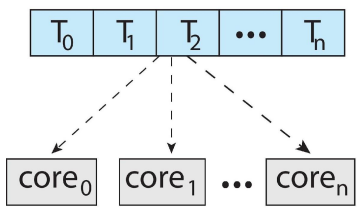
\includegraphics[width = .25\textwidth]{../res/imgs/CPU scheduling/solution_A.png}
    \hspace{2em}
    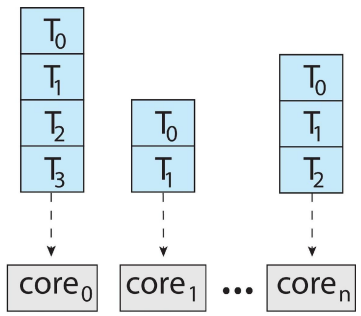
\includegraphics[width = .25\textwidth]{../res/imgs/CPU scheduling/solution_B.png}
    \caption{Ci sono diverse modi per gestire \textit{n} threads con \textit{n} cores.}
    \label{fig:solutionAB}
\end{figure}
Entrambe le soluzioni sono più che lecite anche se ad oggi i sistemi operativi moderni tendono ad usare la seconda in quanto la prima soluzione, essendo si che si ha a che fare con una coda condivisa è complicato gestire la condivisione di tale risorsa tra i cores (problemi di \textit{race conditions}).

\subsection{}
% minuto 7:50 di Lez. 16-03


















% Solution A - Solution B - memory stall - memory stall 2 - two levels scheduling


\section{Scheduling real-time}
\section{Valutazione di un algoritmo}

\todo{Finisci CPU scheduling: parte 2}